% Miktex Beamer template
% Author: Carl Schneider
% University TUDelft
% www.dutiosc.twi.tudelft.nl/~carl/
% Maart 2010

\documentclass{beamer}

\setbeamersize{sidebar width left=0.5cm}
\usepackage[dutch]{babel}
\usepackage{tikz}
\newcommand{\field}[1]{\mathbb{#1}}
\newcommand{\Zset}{\field{Z}}
\mode<presentation>
{\usetheme{Boadilla} % This theme will be adjusted into the TUDelft lay-out
 \setbeamercovered{transparent}}
\definecolor{tudblue}{rgb}{.004,.50,.78} % definition TUDelft blue color
\setbeamercolor{structure}{fg=tudblue}
\setbeamercolor{palette primary}{fg=white,bg=tudblue!85}       % Right field
\setbeamercolor{palette secondary}{fg=white,bg=tudblue!85}     % Middle field
\setbeamercolor{palette tertiary}{fg=tudblue!85,bg=tudblue!85} % Left field
\setbeamersize{text margin left=1cm}
\setbeamersize{text margin right=1cm}

%---------------------------------------------------------------------------------
%  Take attention for the parts you may change. See the comment lines with: %>>>
%---------------------------------------------------------------------------------

%>>> You may change the text in this part {Between brackets}:
%>>> This is for the Title page:
\newcommand*\titel{Project Bolognese}
\newcommand*\subkop{Solving the Bologna process scheduling problem}
\newcommand*\naam{Alon Dolev, Joey Ezechiels, Volker Lanting}
%>>> This is for the frame-title on the "Table of Contents" page:
\newcommand*\titelTOC{Outline}
%>>> This is for the frame-title on the "Table of Contents" page
%>>> when the next subsection will start:
\newcommand*\subsectie{Next subsection}


%%% Not change this part below %%%
%%% Title Page (belongs to theme)%%%
\title{\titel} % This title also appears in the TUDelft bar on the next pages
\author[]{\naam}
\institute[]{\subkop \\ TU Delft}
\date[]{16 november 2012}

\AtBeginSubsection[]
{
\begin{frame}<beamer>\frametitle{\textbf{\LARGE{\textrm{\subsectie}}}}
    \tableofcontents[currentsection,currentsubsection]  % Generation of the Table of Contents
\end{frame}
}
\tikzset{textlabel/.style={color=white}}
%\beamersetuncovermixins{\opaqueness<1>{25}}{\opaqueness<2->{15}} % Transparency Effect
\beamertemplatetransparentcovereddynamicmedium

%==============================================================
\begin{document}
% Adjusting boadilla theme lay-out to TUDelft lay-out:
\setbeamertemplate{sidebar left}  % blue square left above
{\vfill
\rlap{%\hskip0.1cm

\includegraphics[scale=0.33]{TUDelft/beamer-tudelft-bies.jpg} }
\vskip-5pt}

%--------------------------------------------------------------

% Section 0
% Subsection 0
% Page 1
% Title page
\begin{frame}
    \begin{tikzpicture} [remember picture, overlay]
        \node [shift={(0.5 cm,-5.35cm)}]  at (current page.north west)
        {
        \begin{tikzpicture}[remember picture, overlay]
            % These 2 lines you may comment out if you don't want to have a photo on the background of the title page
            \node [shift={(-0.14cm,5.56cm)},right] at (current page.south west)  % background photo
            {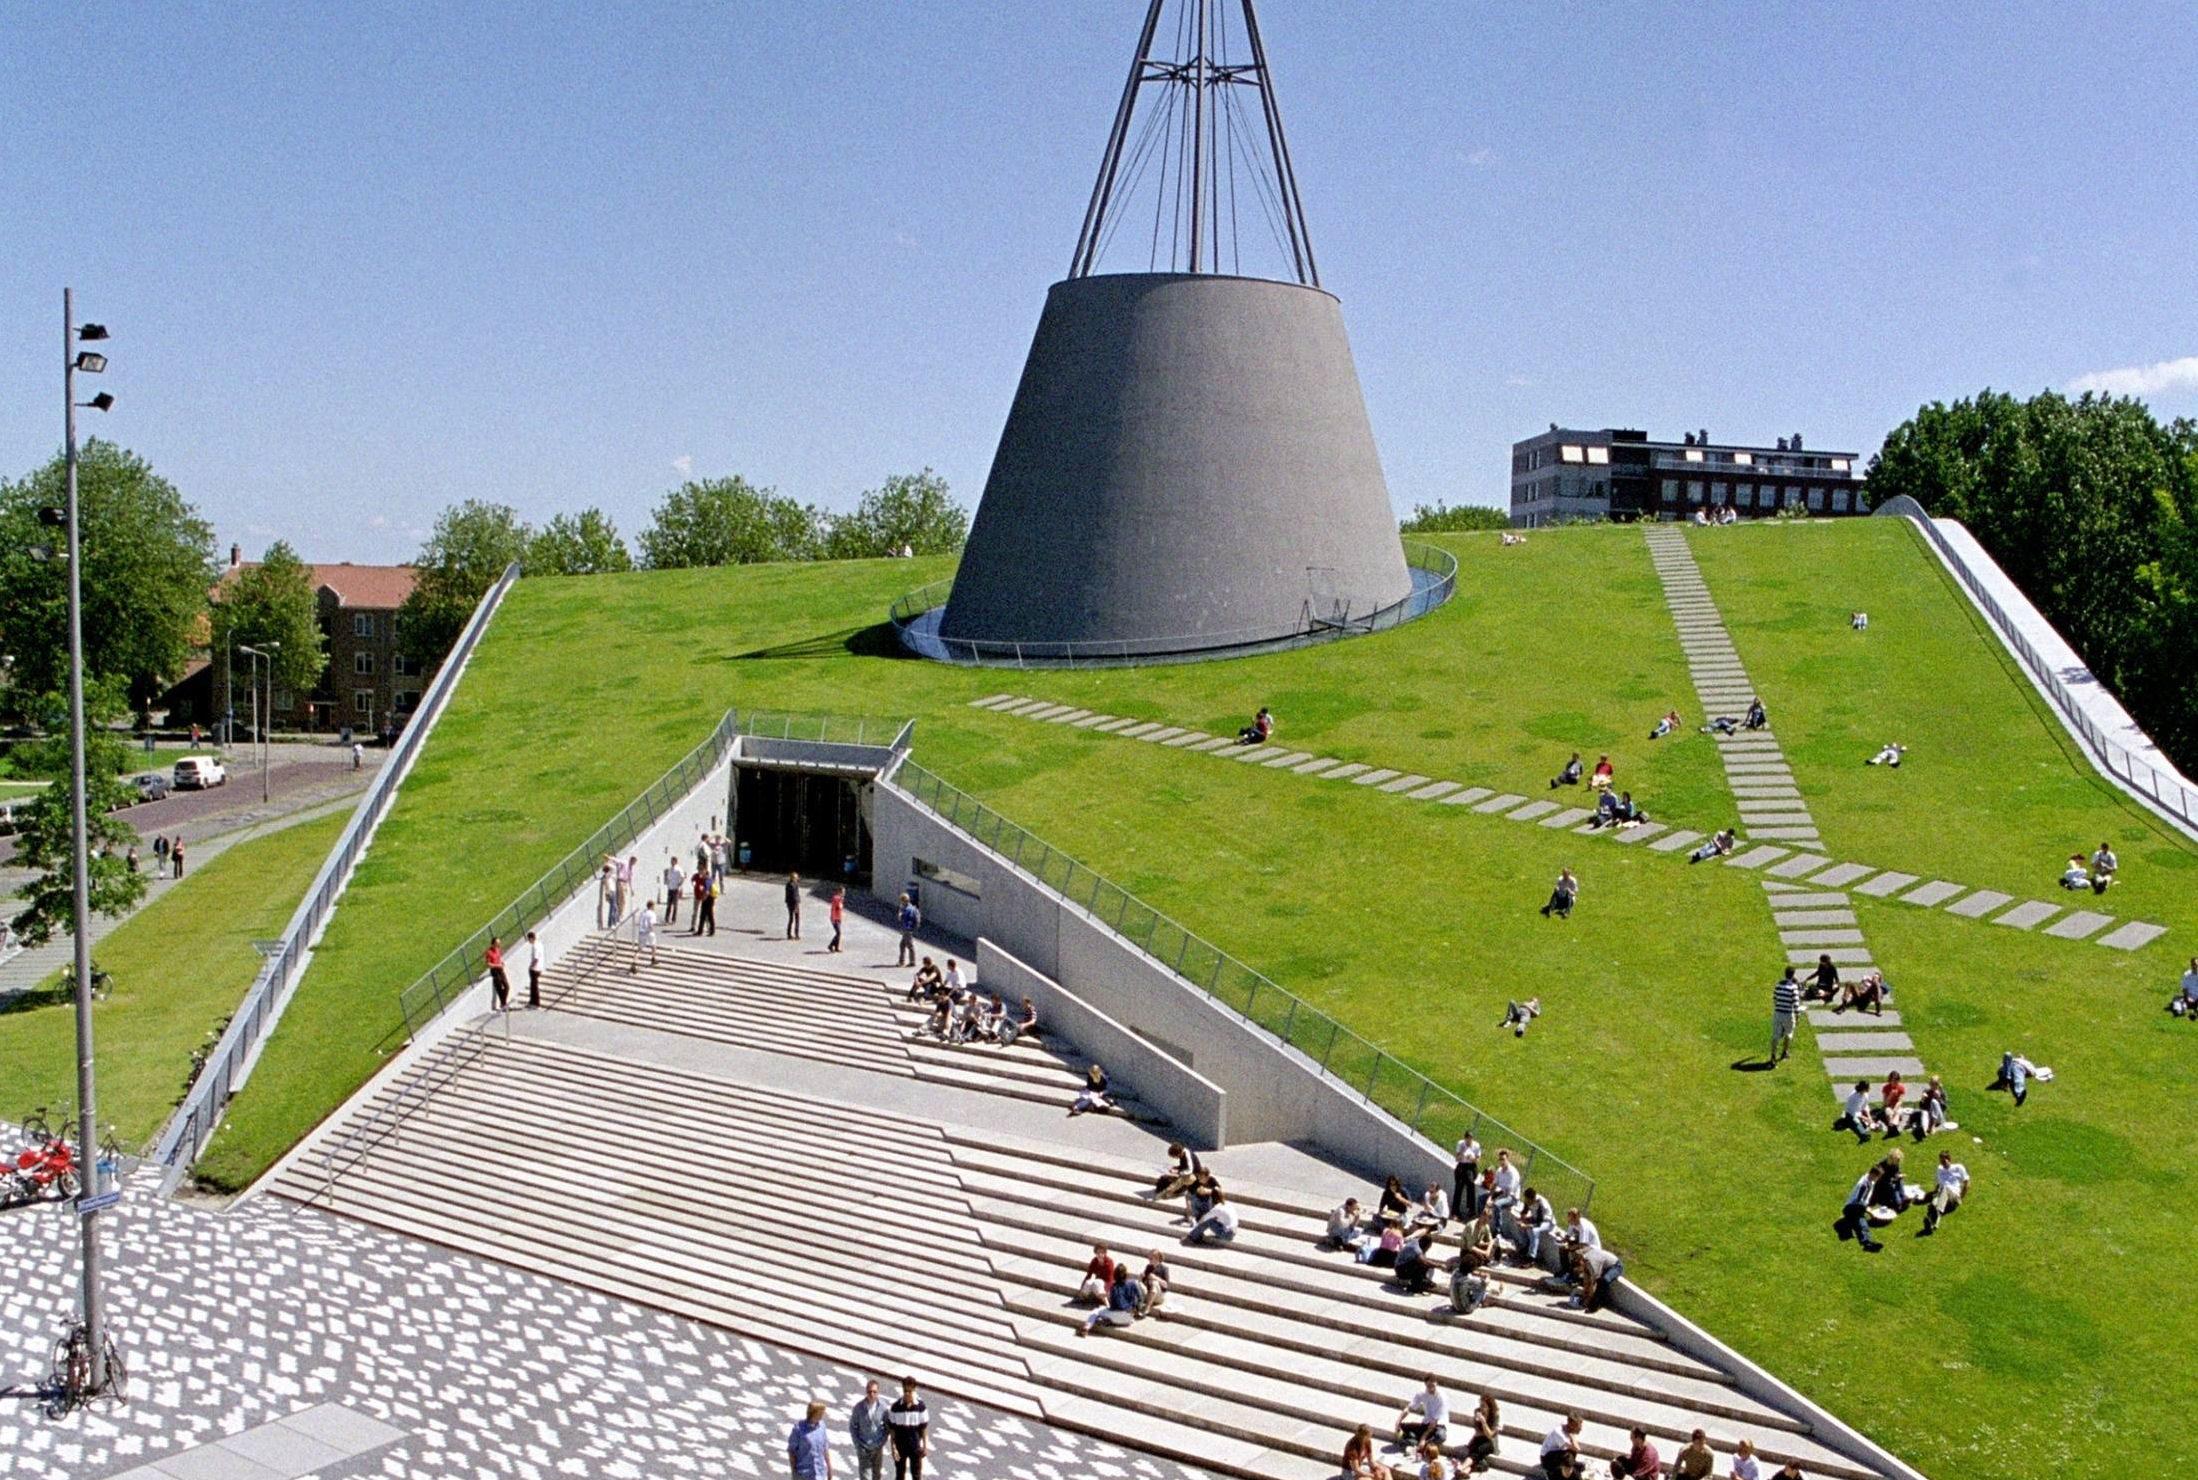
\includegraphics[height=8.65cm]{TUDelft/background-titlepage.jpg}}; % background photo
            \fill [cyan!95!black!70!blue] (0,2.9) -- (0,5.35) -- (-.5,5.35) -- (-.5,2.9) -- cycle ;%squareNorthWest
            \draw [fill=black] (0,0) -- (11,0) -- (11,2.9) -- (0,2.9) -- cycle ;
            \fill [fill=cyan!65!blue!80] (7,-3.9) -- (12.4,-3.9) -- (12.4,-3.65) -- (7,-3.65) -- cycle;
            \node [shift={(0.8cm,-2.9cm)},textlabel,right]  at (current page.north west) {\textbf{\LARGE{\textrm{\titel}}}};
            \node [shift={(0.8cm,-3.5cm)},textlabel,cyan!95!black!70!blue,right]  at (current page.north west)
            {\textbf{\large{\textrm{\subkop}}}};
            \node [shift={(0.8cm,-4.6cm)},textlabel,right]  at (current page.north west)
            {\normalsize{\naam}};
            \node [shift={(0.8cm,-5cm)},textlabel,right]  at (current page.north west)
            {\normalsize{\today}};
        \end{tikzpicture}};
    \end{tikzpicture}
\end{frame}

%--------------------------------------------
%%% Table of contents (TOC)
% The TOC will generated after building your section(s) and subsections
\begin{frame}<beamer>\frametitle{\textbf{\LARGE{\textrm{\titelTOC}}}}
    \begin{tikzpicture}[remember picture, overlay]
        \node [shift={(0.5 cm,-5.35cm)}]  at (current page.north west)
        {
        \begin{tikzpicture}[remember picture, overlay]
            \fill [fill=cyan!65!blue!80] (7,-3.9) -- (12.4,-3.9) -- (12.4,-3.65) -- (7,-3.65) -- cycle;
        \end{tikzpicture}};
    \end{tikzpicture}
    \tableofcontents
\end{frame}
%--------------------------------------------

%--------------------------------------------
%>>> You may change the title-name of the 1st Section: {First section}

\section{First section}

%>>> You may change all the Examples below:
%--------------------------------------------

\subsection{Section 1 - subsection 1}

% Section 1
% Subsection 1
% Page 1
%%% Example:
\begin{frame}\frametitle{\textbf{\LARGE{\textrm{Section 1 - subsection 1 - page 1}}}}
    \begin{example}
        \begin{minipage}{0.6\textwidth}
            % insert picture (pdf file)
            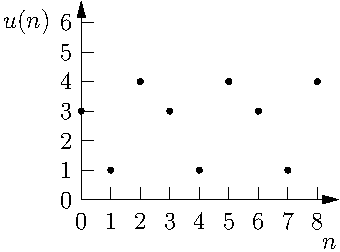
\includegraphics{images/ex1_periodic_number.pdf}
        \end{minipage}
        \centering{$u(n)=[3,1,4]_n$}
    \end{example}
\end{frame}

%--------------------------------------------

% Section 1
% Subsection 1
% Page 2
%%% Example:
\begin{frame}\frametitle{\textbf{\LARGE{\textrm{Section 1 - subsection 1 - page 2}}}}
    \begin{definition}
        Let $n$ be a discrete variable, i.e. $n\in\Zset$.
        A 1-dimensional periodic number is a function that depends periodically on $n$.
        $$
        u(n)=
        [u_0,u_1,\ldots,u_{d-1}]_n=
        \begin{cases}
            u_0 & \mbox{ if $n\equiv 0 \pmod d$} \\
            u_1 & \mbox{ if $n\equiv 1 \pmod d$} \\
            \vdots \\
            u_{d-1} & \mbox{ if $n\equiv d-1 \pmod d$}
        \end{cases}
        $$
        $d$ is called the period.
    \end{definition}
\end{frame}

%--------------------------------------------

% Section 1
% Subsection 1
% Page 3
%%% Example:
\begin{frame}\frametitle{\textbf{\LARGE{\textrm{Section 1 - subsection 1 - page 3}}}}
    \begin{example}
        \centering
        {
        $$
        \begin{array}{rcl}
            f(n)
            &=&
            -\left[\frac{1}{2},\frac{1}{3}\right]_n n^2
            +3n-[1,2]_n
            \\
            &=&
            \begin{cases}
                -\frac{1}{3} n^2 +3n-2
                & \text{ if $n\equiv 0 \pmod 2$} \\
                -\frac{1}{2} n^2 +3n-1
                & \text{ if $n\equiv 1 \pmod 2$}
            \end{cases}
            % &=&
            % -\frac{n^2}{2}+3n-1
            % -\left\{ \frac{n}{2} \right\}
            % \left( \frac{2}{3}n^2+2
            % \right)
        \end{array}
        $$
        \begin{minipage}{0.4\textwidth}
            % insert picture (pdf file)
            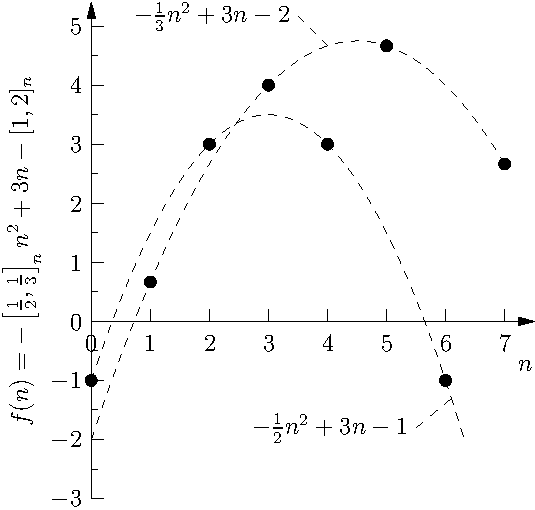
\includegraphics[width=\textwidth]{images/ex2_quasi_polynomial.pdf}
        \end{minipage}
        }
    \end{example}
\end{frame}

%--------------------------------------------

% Section 1
% Subsection 1
% Page 4
%%% Example:
\begin{frame}\frametitle{\textbf{\LARGE{\textrm{Section 1 - subsection 1 - page 4}}}}
    % Show first part of the screen highlighted
    \begin{definition}
        A polynomial in a variable $x$ is a linear combination of powers of $x$:
        $$
        f(x)=\sum_{i=0}^g c_i x^i
        $$
    \end{definition}
    \pause

    % Show second part of the screen highlighted
    \begin{definition}
        A quasi-polynomial in a variable $x$ is a polynomial expression
        with periodic numbers as coefficients:
        $$
        f(n)=\sum_{i=0}^g u_i(n) n^i
        $$
        with $u_i(n)$ periodic numbers.
    \end{definition}
\end{frame}

%--------------------------------------------
%%% Highlighted in the TOC (Second subsection of First section)

\subsection{Section 1 - subsection 2}

% Section 1
% Subsection 2
% Page 1
%%% Example:
\begin{frame}\frametitle{\textbf{\LARGE{\textrm{Section 1 - subsection 2 - page 1}}}}
    \begin{example}
        \begin{columns}
            \column{0.40\textwidth}
            \centering
            \includegraphics<1>[width=\textwidth]{images/ex3a_pp.pdf}
            \includegraphics<2>[width=\textwidth]{images/ex3b_pp.pdf}
            \includegraphics<3>[width=\textwidth]{images/ex3c_pp.pdf}
            \includegraphics<4->[width=\textwidth]{images/ex3d_pp.pdf}
            { \textbf{\small{{$x+y\le p$}}}}
            \column{0.1\textwidth}

            \begin{tabular}{c c}
                $p$ & $f(p)$ \\ \hline
                3 & 5 \\
                \pause
                4 & 8 \\
                \pause
                5 & 10 \\
                \pause
                6 & 13 \\
            \end{tabular}

            \column{0.3\textwidth}
            \pause
            $$
            \frac{5}{2}p+\left[-2,\frac{-5}{2} \right]_p
            $$
        \end{columns}
    \end{example}
\end{frame}

%--------------------------------------------


% Section 1
% Subsection 2
% Page 2
%%% Example:
\begin{frame}\frametitle{\textbf{\LARGE{\textrm{Section 1 - subsection 2 - page 2}}}}
    \begin{itemize}
        \item <1-> The number of integer points in a \alert{parametric polytope} $P_{{p}}$ of dimension $n$
        is expressed as a piecewise a quasi-polynomial of degree $n$ in ${p}$ (Clauss and Loechner).

        \item <2->
        More general \alert{polyhedral counting problems}:\\
        Systems of linear inequalities combined with $\lor, \land, \neg, \forall,$ or $\exists$ (Presburger formulas).
        \item <3->
        Many problems in \alert{static program analysis} can be expressed as polyhedral counting problems.
    \end{itemize}
\end{frame}

%--------------------------------------------
%%% Highlighted in the TOC (Third subsection, First Section)

\subsection{Section 1 - subsection 3}

% Section 1
% Subsection 3
% Page 1
%%% Example:
\begin{frame}\frametitle{\textbf{\LARGE{\textrm{Section 1 - subsection 3 - page 1}}}}
    % Just an example
    A picture made with the package TiKz \\
    \begin{example}
        \centering
        %Number of live elements = quasi-polynomial\\
        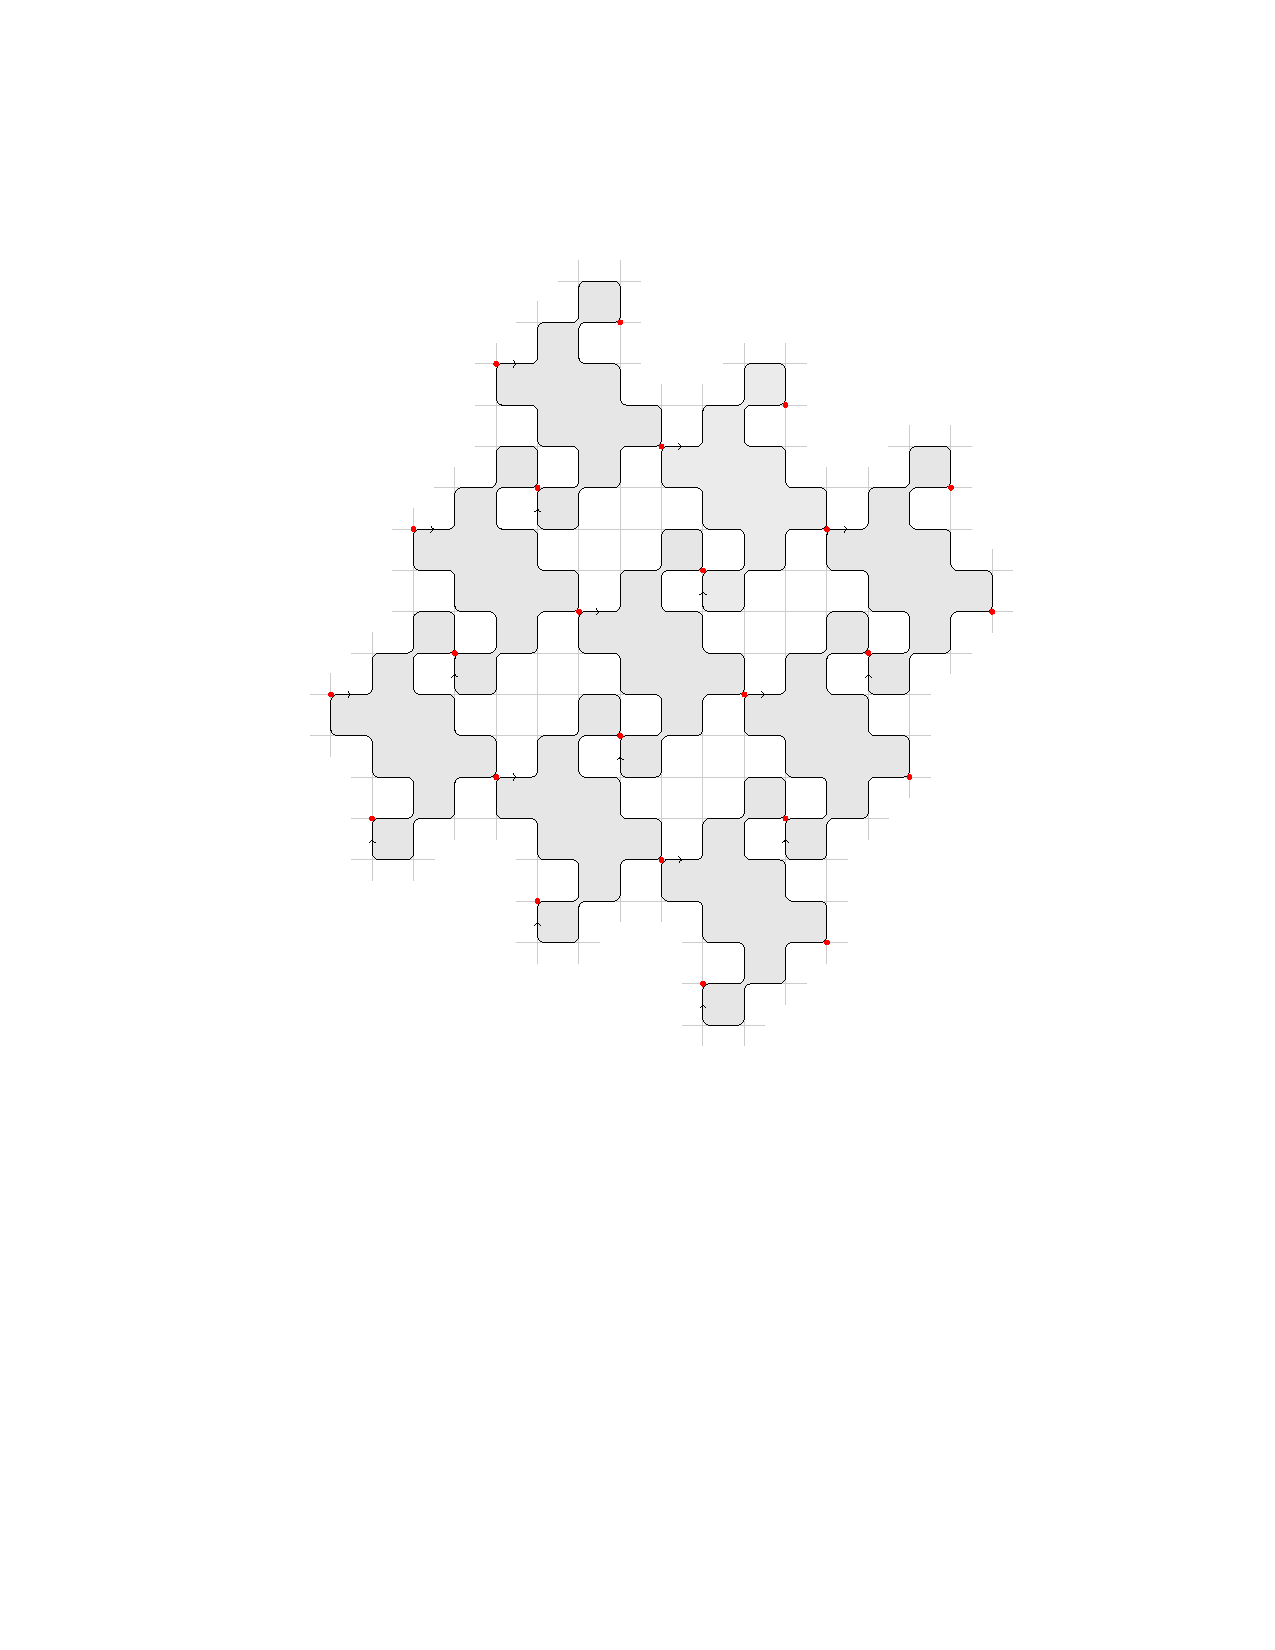
\includegraphics[width=5cm]{images/abadab-anti-theta-01.pdf}
        %$\Downarrow$ \\
        %Memory usage = maximum over all execution points
    \end{example}
\end{frame}

%--------------------------------------------

\section{Second section}

\subsection{Section 2 - subsection 1}

% Section 2
% Subsection 1
% Page 1
%%% Example:
\begin{frame}\frametitle{\textbf{\LARGE{\textrm{Section 2 - subsection 1 - page 1}}}}
    \begin{problem}
        This page gives an example with numbered bullets (enumerate)\\
        in an "Example" window:\\
    \end{problem}

    \begin{example}
        Discrete domain $\Rightarrow$ evaluate in each point \\
        Not possible for \\
        \begin{enumerate}
            \item <1-> parametric domains
            \item <2-> large domains (NP-complete)
        \end{enumerate}
    \end{example}
\end{frame}

%--------------------------------------------

\subsection[]{Section 2 - last subsection}

% Section 2
% Subsection 1
% Page 2
%%% Example:
\begin{frame}\frametitle{\textbf{\LARGE{\textrm{Last page}}}}
    \begin{block}{Summery}
        \centering{End of the beamer demo\\
        with a TUDelft lay-out.\\
        Thank you!}
    \end{block}
\end{frame}
%--------------------------------------------

\end{document} 
